\documentclass{article}
\usepackage{graphicx}
\usepackage{hyperref}

\begin{document}

\begin{figure}[h!]
    \centering
    \includegraphics[width=150px]{https://www.unidformazione.com/wp-content/uploads/2018/04/unipd-universita-di-padova.png}
    \caption{University of Padova Logo}
    \label{fig:unipd-logo}
\end{figure}

\title{FLYDATA - Domain and Data Selection}
\maketitle

\tableofcontents

\section{Group Information}
\textbf{Group Name:} FLYDATA

\textbf{Group Members:}
\begin{enumerate}
    \item Huimin Chen - huimin.chen@studenti.unipd.it - Computer Engineering
    \item Luca Pellegrini - luca.pellegrini.5@studenti.unipd.it - Computer Engineering
    \item Nele Lauryssen - nele.lauryssen@studenti.unipd.it - Computer Science
\end{enumerate}

\section{Selected Datasets}
\begin{enumerate}
    \item \textbf{Airports}
    \begin{itemize}
        \item URL: \href{https://raw.githubusercontent.com/jpatokal/openflights/master/data/airports.dat}{https://raw.githubusercontent.com/jpatokal/openflights/master/data/airports.dat}
        \item Description: Comprehensive dataset containing detailed information about airports worldwide.
        \item Relevance: Starting and ending points of flights; potential for analyzing airport traffic.
        \item Note: Extended version available at \href{https://github.com/jpatokal/openflights/blob/master/data/airports-extended.dat}{https://github.com/jpatokal/openflights/blob/master/data/airports-extended.dat}
    \end{itemize}
    
    \item \textbf{Planes}
    \begin{itemize}
        \item URL: \href{https://github.com/jpatokal/openflights/blob/master/data/planes.dat}{https://github.com/jpatokal/openflights/blob/master/data/planes.dat}
        \item Description: List of planes with Name, IATA code, ICAO code.
        \item Relevance: Essential for flight operations.
    \end{itemize}
    
    \item \textbf{Airlines}
    \begin{itemize}
        \item URL: \href{https://raw.githubusercontent.com/jpatokal/openflights/master/data/airlines.dat}{https://raw.githubusercontent.com/jpatokal/openflights/master/data/airlines.dat}
        \item Description: List of airlines with detailed information.
        \item Relevance: Flight operators; potential for performance analysis.
    \end{itemize}
    
    \item \textbf{Routes}
    \begin{itemize}
        \item URL: \href{https://raw.githubusercontent.com/jpatokal/openflights/master/data/routes.dat}{https://raw.githubusercontent.com/jpatokal/openflights/master/data/routes.dat}
        \item Description: List of routes with comprehensive flight planning information.
        \item Relevance: Connects airports; provides insights into flight planning and route popularity.
    \end{itemize}
    
    \item \textbf{Countries}
    \begin{itemize}
        \item URL: \href{https://raw.githubusercontent.com/jpatokal/openflights/master/data/countries.dat}{https://raw.githubusercontent.com/jpatokal/openflights/master/data/countries.dat}
        \item Description: List of countries with ISO and DAFIF codes.
        \item Relevance: Contextual information for airports; potential impact on flight quantity and route planning.
    \end{itemize}
    
    \item \textbf{Cities}
    \begin{itemize}
        \item URL: \href{https://simplemaps.com/data/world-cities}{https://simplemaps.com/data/world-cities}
        \item Description: List of cities with geographic and demographic information.
        \item Relevance: Context for airports; potential correlation between population and route numbers.
    \end{itemize}
    
    \item \textbf{Airline Service Quality Performance 234 (On-Time performance data)}
    \begin{itemize}
        \item URL: \href{https://www.bts.gov/browse-statistical-products-and-data/bts-publications/airline-service-quality-performance-234-time}{https://www.bts.gov/browse-statistical-products-and-data/bts-publications/airline-service-quality-performance-234-time}
        \item Relevance: Insights into airline performance and on-time statistics.
    \end{itemize}
    
    \item \textbf{Runways}
    \begin{itemize}
        \item URL: \href{https://ourairports.com/data/}{https://ourairports.com/data/}
        \item Description: Detailed runway information including dimensions and characteristics.
        \item Relevance: Critical for understanding airport capacity and operations.
    \end{itemize}
    
    \item \textbf{Frequencies}
    \begin{itemize}
        \item URL: \href{https://ourairports.com/data/}{https://ourairports.com/data/}
        \item Description: List of airport frequencies.
        \item Relevance: Important for air traffic control and communication.
    \end{itemize}
    
    \item \textbf{Delay Causes}
    \begin{itemize}
        \item URL: \href{https://www.kaggle.com/datasets/sriharshaeedala/airline-delay}{https://www.kaggle.com/datasets/sriharshaeedala/airline-delay} or \href{https://www.transtats.bts.gov/ot_delay/ot_delaycause1.asp}{https://www.transtats.bts.gov/ot_delay/ot_delaycause1.asp}
        \item Description: Detailed information on flight delays and their causes.
        \item Relevance: Critical for analyzing and understanding flight delays.
    \end{itemize}
\end{enumerate}

\section{Model Design}

\begin{figure}[h!]
    \centering
    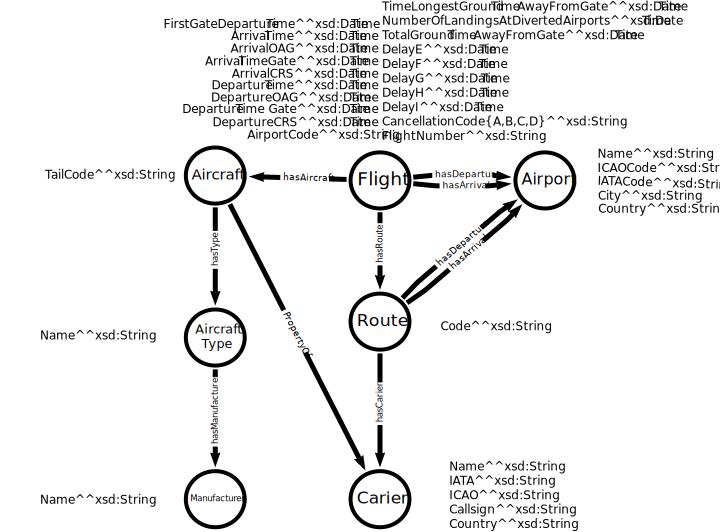
\includegraphics[width=\textwidth]{GraphComp.svg}
    \caption{Graph Component Model}
    \label{fig:graph-comp-model}
\end{figure}

\subsection{Main Entities}
\begin{enumerate}
    \item Flight: flight number, departure time, arrival time, departure airport, arrival airport, route, aircraft etc.
    \item Airport: name, code, etc.
    \item Route: name
    \item Aircraft: name, code, etc.
    \item AircraftType: name, etc.
    \item Manufacturer: name, etc.
    \item Carrier: name, code, etc.
\end{enumerate}

\subsection{Relationships}
\begin{enumerate}
    \item Flight - Airport: "hasDeparture"
    \item Flight - Airport: "hasArrival"
    \item Flight - Route: "hasRoute"
    \item Flight - Aircraft: "hasAircraft"
    \item Aircraft - AircraftType: "hasType"
    \item AircraftType - Manufacturer: "hasManufacturer"
    \item Route - Airport: "hasDeparture"
    \item Route - Airport: "hasArrival"
    \item Route - Carrier: "hasCarrier"
    \item Aircraft - Carrier: "PropertyOf"
\end{enumerate}

This model enables flexible querying and analysis, such as:
\begin{itemize}
    \item Finding all routes from a specific airport
    \item Analyzing airline operations across different countries
    \item Exploring the relationship between city population and airport traffic
\end{itemize}

The model is extensible to include additional entities like Planes, Runways, and Delay Causes for more detailed analysis.

\section{Main Challenges}

\begin{enumerate}
    \item Data Integration: Combining multiple datasets with varying formats and structures.
    \item Data Quality: Ensuring accuracy and completeness across all datasets.
    \item Data Volume: Managing large amounts of frequently updated data.
    \item Temporal Alignment: Dealing with time zone differences and aligning data from different periods.
    \item Relationship Mapping: Establishing correct relationships between entities across datasets.
    \item Data Cleaning: Handling missing values, duplicates, and errors in raw datasets.
    \item Performance Optimization: Designing efficient queries and data structures for complex analyses.
\end{enumerate}

\section{Main Characteristics}

\begin{enumerate}
    \item Global Coverage: Comprehensive worldwide information on air travel.
    \item Multi-dimensional: Spans geographic, operational, and performance-related aspects.
    \item Interconnected: Allows for complex analyses across different entities in the air travel ecosystem.
    \item Wide Application: Useful for flight planning, route optimization, performance analysis, and customer service.
\end{enumerate}

\end{document}
